\section{Lecture 6 | Value Function Approximation}
Reinforcement learning can be used to solve large scale problems.
\begin{itemize}
    
    \item Backgammon: \(10^{20}\) states
    \item Computer Go: \(10^{170}\) states
    \item Helicopter control: continous state space 
\end{itemize}
Thus, we need to scale up the model-free methods for prediction and control.

The solution for the large MDPsis to estimate with \emph{function approximation}.
\[
    \begin{aligned}
        \hat{v}(s,\mathbf{w}) &\approx v_{\pi}(s) \\
        \hat{q}(s,a,\mathbf{w}) &\approx q_{\pi}(s,a)
    \end{aligned}  
\]
where \(\mathbf{w}\) is the weight vector of the function approximator, which is updated 
using say MC or TD learning. The hope is that the function approximator will generalise
from the states it has seen to the states it has not seen.

\begin{figure}[H]
    \centering
    \begin{subfigure}[b]{0.25\textwidth}
        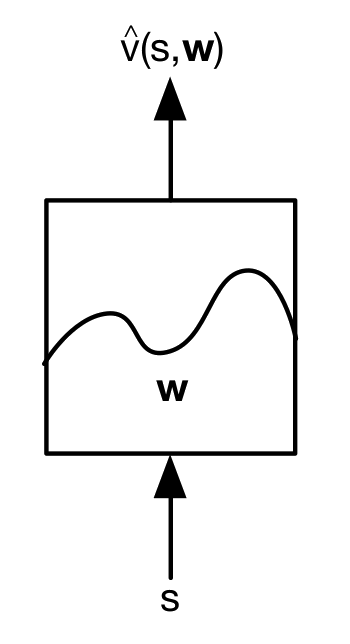
\includegraphics[width=\textwidth]{figures/fa-v.png}
        \caption{Value FA}
        \label{fig:fav}
    \end{subfigure}
    \begin{subfigure}[b]{0.25\textwidth}
        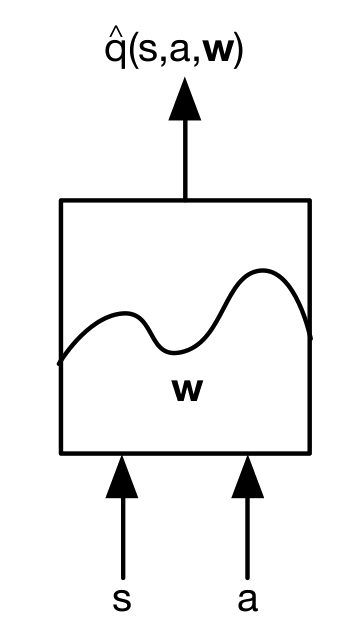
\includegraphics[width=\textwidth]{figures/fa-ain.png}
        \caption{Action In Action Value FA}
        \label{fig:faain}
    \end{subfigure}
    \begin{subfigure}[b]{0.3\textwidth}
        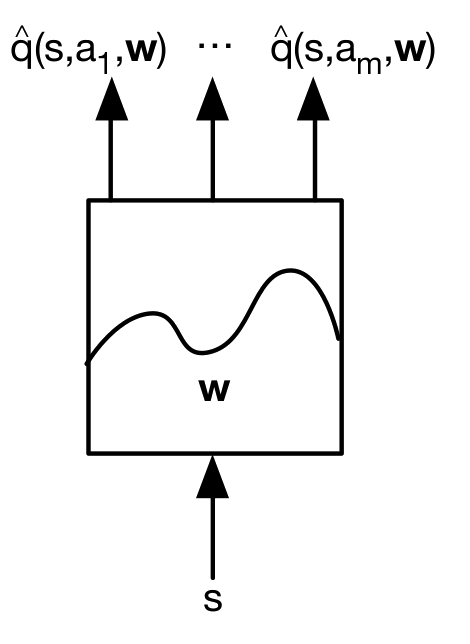
\includegraphics[width=\textwidth]{figures/fa-aout.png}
        \caption{Action Out Action Value FA}
        \label{fig:faaout}
    \end{subfigure}
    \caption{Different types of Function Approximators (FA)}
\end{figure}
We will be using differentiable function approximators, thus we can use gradient descent
to tune the parametrc weight vector \(\mathbf{w}\).

\subsection{Incremental Methods}

\subsubsection*{Gradient Descent}
Let \(J(\mathbf{w})\) be a differntiable function of the parameter vector \(\mathbf{w}\).
Let the gradient of the function \(J(\mathbf{w})\) be \(\nabla J(\mathbf{w})\), and be 
defined as:
\[
    \nabla J(\mathbf{w}) = \begin{bmatrix}
        \frac{\partial J(\mathbf{w})}{\partial w_1} \\
        \frac{\partial J(\mathbf{w})}{\partial w_2} \\
        \vdots \\
        \frac{\partial J(\mathbf{w})}{\partial w_n} \\
    \end{bmatrix}
\]
The parameter vector \(\mathbf{w}\) is updated as:
\[
    \Delta \mathbf{w} = -\frac{1}{2} \alpha \nabla J(\mathbf{w})
\]
where \(\alpha\) is the learning rate or step size. Follwoiu this update rule, we can
find a minimum of the function \(J(\mathbf{w})\).

\subsubsection{Value Function Approximation via Stochastic Gradient Descent}
The goal is to find the parameter vector \(\mathbf{w}\) that minimises the mean squared
error between approximate value function \(\hat{v}(s,\mathbf{w})\) and the true value 
function \(v_{\pi}(s)\)
\[
    \implies J(\mathbf{w}) = \mathbb{E}_{\pi}\left[ 
        \left( 
            v_{\pi}(s) - \hat{v}(s,\mathbf{w})
         \right)^{2} 
     \right] 
\]
Thus, via gradient descent, we can update the parameter vector \(\mathbf{w}\) as:
\[
    \begin{aligned}
        \Delta \mathbf{w} &= -\frac{1}{2} \alpha \nabla J(\mathbf{w}) \\
        &= \alpha \mathbb{E}_{\pi} \left[ 
            (v_{\pi}(s) - \hat{v}(s,\mathbf{w})) \nabla \hat{v}(s,\mathbf{w})
         \right] 
    \end{aligned}  
\]
Note: this assumes the value function \(v_{\pi}(s)\) is known.
Stochatisc gradient descent samples the gradient giving:
\[
    \Delta \mathbf{w} = \alpha \left[ 
        v_{\pi}(s) - \hat{v}(s,\mathbf{w})
     \right] \nabla \hat{v}(s,\mathbf{w})  
\]
Thus, the expected update is the full gradient update.

\subsubsection{Examples of Function Approximators}
\begin{itemize}
    \item Feature Vector: Represent the state as a feature vector \(\mathbf{x}(S)\)
    \[
        \mathbf{x}(S) = \begin{pmatrix}
            x_1(S) \\
            x_2(S) \\
            \vdots \\
            x_n(S) \\
        \end{pmatrix}  
    \]
    The examples can be: the distance of a robot from some features or landmarks, or piece
    and pawn configuration in chess etc.
    \item Linear Value Function Approximation: Represent value function as a linear
    combination of features.
    \[
        \hat{v}(s,\mathbf{w}) = \mathbf{x}(s)^{\top}  \mathbf{w} = \sum_{j=1}^{n} x_j(s) w_j  
    \]
    Since the objective function is quadratic in parameter vector \(\mathbf{w}\):
    \[
        J(\mathbf{w}) = \mathbb{E}_{\pi}\left[ 
            \left( 
                v_{\pi}(s) - \hat{v}(s,\mathbf{w})
             \right)^{2} 
         \right]
    \]
    stocahtisc gradient descent converges to the global minimum. The update rule is given
    as:
    \[
        \begin{aligned}
            \nabla_{\mathbf{w}} \hat{v}(s,\mathbf{w}) &= \mathbf{x}(s) \\
            \Delta \mathbf{w} &= \alpha \left[ 
                v_{\pi}(s) - \hat{v}(s,\mathbf{w})
             \right] \mathbf{x}(s)
        \end{aligned}
    \]
    \item Table Lookup Features: Table lookup is a spaecia case of linear value function. Thus,
    all of the algorithms used till now, can be implemented using table lookup features.
    The table loopup features are given as:
    \[
        \mathbf{x}(s) = \begin{pmatrix}
            \mathbb{I}(s = s_1) \\
            \mathbb{I}(s = s_2) \\
            \vdots \\
            \mathbb{I}(s = s_n) \\
        \end{pmatrix}
    \]
    The parameter vector \(\mathbf{w}\) is the vector of values for each state:
    \[
        \mathbf{w} = \begin{pmatrix}
            v_{\pi}(s_1) \\
            v_{\pi}(s_2) \\
            \vdots \\
            v_{\pi}(s_n) \\
        \end{pmatrix}
    \]

\end{itemize}

\subsection{Incremental Prediction Algorithms}
We will now replace the true value function \(v_{\pi}(s)\) with the appropirate target
for \(v_{\pi}(s)\). The target for \(v_{\pi}(s)\) is caluclated as:
\begin{itemize}
    \item Monte Carlo: the tagert is the return \(G_t\)
    \[
        \Delta \mathbf{w} = \alpha \left[ 
            G_t - \hat{v}(S_t,\mathbf{w})
         \right] \nabla \hat{v}(S_t,\mathbf{w})  
    \]
    \item TD(0): the target is the TD target \(R_{t+1} + \gamma \hat{v}(S_{t+1},\mathbf{w})\)
    \[
        \Delta \mathbf{w} = \alpha \left[ 
            R_{t+1} + \gamma \hat{v}(S_{t+1},\mathbf{w}) - \hat{v}(S_t,\mathbf{w})
         \right] \nabla \hat{v}(S_t,\mathbf{w})
    \]
    \item TD(\(\lambda\)): the target is the \(\lambda\)-return  \(G_t^{\lambda}\)
    \[
        \Delta \mathbf{w} = \alpha \left[ 
            G_t^{\lambda} - \hat{v}(S_t,\mathbf{w})
         \right] \nabla \hat{v}(S_t,\mathbf{w})
    \]
    where,
    \[
        G_t^{\lambda} = (1-\lambda) \sum_{n=1}^{\infty} \lambda^{n-1} G_{t:t+n}  
    \]
\end{itemize} 

\subsubsection{Monte Carlo with Value Function Approximation}
The retuen \(G_t\) is an unbiased, noisy sample of the true value \(v_{\pi}(S_t)\). Thus the
supervised learning can be applied to the trajectory or \emph{traning data}:
\[
    \langle S_1,G_1 \rangle, \langle S_2,G_2 \rangle, \dots, \langle S_T,G_T \rangle
\]
For example using using linear value function approximation, the update rule is given as:
\[
    \Delta \mathbf{w} = \alpha \left[ 
        G_t - \hat{v}(S_t,\mathbf{w})
     \right] \mathbf{x}(S_t)
\]
Since the monte carlo method is unbiased, the update rule converges to some global minimum.
The monte carlo method will still converege to some local minimum even when using non-linear
function approximators.

\subsubsection{TD(0) with Value Function Approximation}
The TD target \(R_{t+1} + \gamma \hat{v}(S_{t+1},\mathbf{w})\) is a biased sample of the
true value \(v_{\pi}(S_t)\). Thus, the supervised learning can be applied to the trajectory
or \emph{training data}:
\[
    \langle S_1,R_2 + \gamma \hat{v}(S_2,\mathbf{w}) \rangle, \langle S_2,
    R_3 + \gamma \hat{v}(S_3,\mathbf{w}) \rangle, \dots, \langle S_T,R_{T+1} \rangle
\]
For example using using linear value function approximation, the update rule is given as:
\[
    \begin{aligned}
        \Delta \mathbf{w} &= \alpha \left[ 
            R_{t+1} + \gamma \hat{v}(S_{t+1},\mathbf{w}) - \hat{v}(S_t,\mathbf{w})
         \right] \mathbf{x}(S_t)  \\
         & = \alpha \delta \mathbf{x}(S_t)
    \end{aligned}
\]
The linear TD(0) converges close to the global minimum.

\subsubsection{TD(\(\lambda\)) with Value Function Approximation}
The \(\lambda\)-return \(G_t^{\lambda}\) is a biased sample of the true value \(v_{\pi}(S_t)\).
Thus, the supervised learning can be applied to the trajectory or \emph{training data}:
\[
    \langle S_1,G_1^{\lambda} \rangle, \langle S_2,G_2^{\lambda} \rangle, \dots, \langle S_T,
    G_T^{\lambda} \rangle
\]
Forward view linear TD(\(\lambda\)):
\[
    \begin{aligned}
        \Delta \mathbf{w} &= \alpha \left[ 
            G_t^{\lambda} - \hat{v}(S_t,\mathbf{w})
         \right]\nabla \hat{v}(S_t,\mathbf{w})  \\
         & = \alpha \left[ 
            G_t^{\lambda} - \hat{v}(S_t,\mathbf{w})
         \right]  \mathbf{x}(S_t)
    \end{aligned}
\]
Backward view linear TD(\(\lambda\)):
\[
    \begin{aligned}
        \delta _t &= R_{t+1} + \gamma \hat{v}(S_{t+1},\mathbf{w}) - \hat{v}(S_t,\mathbf{w}) \\
        E_t &= \gamma \lambda E_{t-1} + \mathbf{x}(S_t) \\
        \implies \Delta \mathbf{w} &= \alpha \delta_t E_t
    \end{aligned}
\]

\subsection{Incremental Control Algorithms}
\begin{itemize}
    \item Policy Evalution: approximate policy evaluation of the state action value function:
    \[
        \hat{q}(s,a,\mathbf{w}) \approx q_{\pi}(s,a)
    \]
    \item Policy Improvement: \(\epsilon\)-greedy policy improvement 
\end{itemize}
In practice, with the control case, we will typically end up with the algorithms that will 
oscialte around.

Thus, we will need to do the same this done in the state value funtion case to the state
action value function.

Thus we have:
Approximate the action value function:
\[
    \hat{q}(s,a,\mathbf{w}) \approx q_{\pi}(s,a)  
\]    
Minmise the mean squared error between the approximate action value function \(\hat{q}(s,a,
\mathbf{w})\) and the true action value function \(q_{\pi}(s,a)\):
\[
    J(\mathbf{w}) = \mathbb{E}_{\pi}\left[ 
        \left( q_{\pi}(s,a) - \hat{q}(s,a,\mathbf{w}) \right)^2
     \right] 
\]
Using stocahtisc gradient descent, we can update the parameter vector \(\mathbf{w}\) as:
\[
\Delta \mathbf{w} = \alpha \left[ 
    q_{\pi}(s,a) - \hat{q}(s,a,\mathbf{w})
 \right] \nabla \hat{q}(s,a,\mathbf{w})
\]

For example, using linear value function approximation. Thus, the state and action can be
represented by a feature vector:
\[
    \mathbf{x}(s,a) = \begin{pmatrix}
        x_1(s,a) \\
        x_2(s,a) \\
        \vdots \\
        x_n(s,a) \\
    \end{pmatrix}  
\]
hence, the action value function can be represented by a linear combination of features:
\[
    \hat{q}(s,a,\mathbf{w}) = \mathbf{x}(s,a)^{\top} \mathbf{w} = \sum_{j=1}^{n} x_j(s,a) w_j
\]
Thus, the update rule is given using stocahtisc gradient descent:
\[
\begin{aligned}
    \nabla_{\mathbf{w}} \hat{q}(s,a,\mathbf{w}) &= \mathbf{x}(s,a) \\
    \Delta \mathbf{w} &= \alpha \left[ 
        q_{\pi}(s,a) - \hat{q}(s,a,\mathbf{w})
     \right] \mathbf{x}(s,a)
\end{aligned}
\]

Similar to the case of function approximation for state value function, we can use the target
for the action value function as per the algorithm used:
\begin{itemize}
    \item Monte Carlo: the tagert is the return \(G_t\)
    \[
        \Delta \mathbf{w} = \alpha \left[ 
            G_t - \hat{q}(S_t,A_t,\mathbf{w})
         \right] \nabla \hat{q}(S_t,A_t,\mathbf{w})  
    \]
    \item TD(0): the target is the TD target \(R_{t+1} + \gamma \hat{q}(S_{t+1},A_{t+1},
    \mathbf{w})\)
    \[
        \Delta \mathbf{w} = \alpha \left[ 
            R_{t+1} + \gamma \hat{q}(S_{t+1},A_{t+1},\mathbf{w}) - \hat{q}(S_t,A_t,
            \mathbf{w})
         \right] \nabla \hat{q}(S_t,A_t,\mathbf{w})
    \]
    \item TD(\(\lambda\)): the target is the \(\lambda\)-return  \(G_t^{\lambda}\)
    \[
        \Delta \mathbf{w} = \alpha \left[ 
            G_t^{\lambda} - \hat{q}(S_t,A_t,\mathbf{w})
         \right] \nabla \hat{q}(S_t,A_t,\mathbf{w})
    \]
    where,
    \[
        G_t^{\lambda} = (1-\lambda) \sum_{n=1}^{\infty} \lambda^{n-1} G_{t:t+n}  
    \]
    This is the forward view TD(\(\lambda\)) algorithm.

    \item Backward view TD(\(\lambda\)):
    \[
        \begin{aligned}
            \delta _t &= R_{t+1} + \gamma \hat{q}(S_{t+1},A_{t+1},\mathbf{w}) - \hat{q}(S_t,
            A_t,\mathbf{w}) \\
            E_t &= \gamma \lambda E_{t-1} + \mathbf{x}(S_t,A_t) \\
            \implies \Delta \mathbf{w} &= \alpha \delta_t E_t
        \end{aligned}
    \]
\end{itemize}

\subsubsection{Convergence of Algorithms}
\begin{table}[H]
    \centering
    \caption{Convergence of Prediction Algorithms}
    \label{tab:convergence-prediction}
    \begin{tabular}{ccccc}
    \hline
    On/Off-Policy               & Algorithm   & Table Lookup & Linear     & Non Linear \\ \hline
    \multirow{3}{*}{On Policy}  & MC          & \checkmark   & \checkmark & \checkmark \\ \cline{2-5} 
                                & TD          & \checkmark   & \checkmark & \xmark     \\ \cline{2-5} 
                                & Gradient TD & \checkmark   & \checkmark & \checkmark \\ \hline
    \multirow{3}{*}{Off Policy} & MC          & \checkmark   & \checkmark & \checkmark \\ \cline{2-5} 
                                & TD          & \checkmark   & \xmark     & \xmark     \\ \cline{2-5} 
                                & Gradient TD & \checkmark   & \checkmark & \checkmark \\ \hline
    \end{tabular}
\end{table}
\begin{table}[H]
    \centering
    \caption{Convergence of Control Algorithms}
    \label{tab:convergence-control}
    \begin{tabular}{cccc}
    \hline
    Algorithm           & Table Lookup & Linear       & Non Linear \\ \hline
    MC                  & \checkmark   & (\checkmark) & \xmark     \\ \hline
    SARSA               & \checkmark   & (\checkmark) & \xmark     \\ \hline
    Q Learning          & \checkmark   & \xmark       & \xmark     \\ \hline
    Gradient Q Lwarning & \checkmark   & \checkmark   & \xmark     \\ \hline
    \end{tabular}
    \end{table}

\subsection{Batch Reinforcement Learning}
Gradient descent methods ares imple and appeling, but they ar enot sample efficient. So, the idea of the 
batch methids is to fit the best fitting value function across all of the trainig data of the agent i.e. the
history of the agent. One of the defination of the best fit is the least sqaures fit.

\subsubsection{Least Squares Prediction}
Given a value function approximaion, \(v(s,\mathbf{w}) \approx v_{\pi}(s)\), and the experience \(\mathcal{D}\)
consiting of state vaue pairs :
\[
    \mathcal{D} =  \langle S_1,v_1^{\pi} \rangle, \langle S_2,v_2^{\pi} \rangle, \dots, \langle S_T,v_T^{\pi} \rangle 
\] 
find the parameters \(\mathbf{w}\) that minimises the mean squared error between the approximate value function
\(v(s,\mathbf{w})\) and the true value function \(v_{\pi}(s)\) or the target value \(v_t^{\pi}\):
\[
    \begin{aligned}
        LS(\mathbf{w}) &= \sum_{t=1}^{T} \left[ 
            v_t^{\pi} - v(s_t,\mathbf{w})
         \right]^2 \\
         &= \mathbb{E}_{\mathcal{D}} \left[ 
            \left( 
                v^{\pi} - v(s,\mathbf{w})
             \right)^2
          \right]
    \end{aligned}
\]

\subsubsection{Stochastic Gradient Descent with Experience Replay}
Given, experince consisteing of state value pairs:
\[
    \mathcal{D} =  \langle S_1,v_1^{\pi} \rangle, \langle S_2,v_2^{\pi} \rangle, \dots, \langle S_T,v_T^{\pi} \rangle
\]
Sample state value pair \(\langle S_t,v_t^{\pi} \rangle\) from the experience \(\mathcal{D}\). Then, update the
parameter vector \(\mathbf{w}\) with the follwoing update rule:
\[
    \Delta \mathbf{w} = \alpha \left[ 
        v^{\pi} - v(s,\mathbf{w})
     \right] \nabla v(s,\mathbf{w})  
\]
This update rule converges to least squares solution:
\[
    \mathbf{w}^{\pi} = \argmin_{\mathbf{w}} LS(\mathbf{w})  
\]

\subsubsection{Experience Replay in Deep Q-Networks (DQN)}
DQN uses experience replay and fixed Q-targets to stabilise the learning.
\begin{itemize}
    \item Taklee action \(a_t\) according to \(\epsilon\)-greedy policy
    \item Store the transition \(\langle S_t,A_t,R_{t+1},S_{t+1} \rangle\) in the replay
    buffer \(\mathcal{D}\) 
    \item Sample random minibatch of transitions \(\langle S,A,R,S^{\prime} \rangle\) from \(\mathcal{D}\)
    \item Compute Q-learning targets with fixed Q-targets wrt to old parametrs \(\mathbf{w}^{-}\):
    \item Optimse the MSE between Q-network and Q-learning targets:
    \[
        \mathcal{L}_i(\mathbf{w}_i) = \mathbb{E}_{S,A,R,S^{\prime} \sim \mathcal{D}_i} \left[ 
            \left( 
                y_i - Q(S,A;\mathbf{w}_i)
             \right)^2
         \right]
    \]
    where \(y_i = R + \gamma \max\limits_{a^{\prime}} Q(S^{\prime},a^{\prime};\mathbf{w}_i^{-})\)

\end{itemize}

\subsubsection{Linear Least Squares Prediction}
Experience Replay finds the least sqaures solutions, but it may take many many iterations, and thus it is not
sample efficient. Using linear value function approximation, \(\hat{v}(s,\mathbf{w}) = \mathbf{x}(s)^{\top}
\mathbf{w}\), we can find a closed form least squares solution.

At minimum of LS(\(\mathbf{w}\)), the expected update must be zero:
\[
    \begin{aligned}
        \mathbb{E}_{\mathcal{D}} \left[ \Delta \mathbf{w} 
         \right]  &= 0 \\
         \alpha \sum_{t=1}^T \mathbf{x}(s_t)(v_t^{\pi} - \mathbf{x}(s_t)^{\top} \mathbf{w}) &= 0 \\
         \sum_{t=1}^T \mathbf{x}(s_t) v_t^{\pi} &= \sum_{t=1}^T \mathbf{x}(s_t) \mathbf{x}
         (s_t)^{\top} \mathbf{w} \\
         \implies  \mathbf{w} &= \left( \sum_{t=1}^T \mathbf{x}(s_t) \mathbf{x}(s_t)^{\top} \right)^{-1}
          \sum_{t=1}^T \mathbf{x}(s_t) v_t^{\pi}
    \end{aligned}
\]

SInce we dont know the true value function \(v_{\pi}(s)\), we can use the noisy or biased estimate of
\(v_t^{\pi}\) as the target:
\begin{itemize}
    \item LSMC : Least Squares Monte Carlo use the return \(G_t\) as the target:
    \[
        v_t^{\pi} \approx  G_t
    \]
    \item LSTD(0) : Least Squares Temporal Difference uses the TD target:
    \[
        v_t^{\pi} \approx R_{t+1} + \gamma \hat{v}(S_{t+1},\mathbf{w})  
    \]
    \item LS(\(\lambda\)) : Least Squares TD(\(\lambda\)) uses the \(\lambda\)-return \(G_t^{\lambda}\) as the
    target:
    \[
        v_t^{\pi} \approx G_t^{\lambda}
    \]
\end{itemize}